\documentclass {article}

\usepackage [utf8]{inputenc}
\usepackage{lmodern}
\usepackage[T1]{fontenc}
\usepackage {graphicx}
\usepackage[official]{eurosym}

\renewcommand {\contentsname} {Indice}

\title {{\Huge Bitcoin, blockchain, crypto}}

\author {Carlomaria Occhipinti\\Liceo Scientifico Arturo Tosi}

\date {Giugno 2018}


\begin {document}


\maketitle

\pagenumbering {gobble}

\newpage

\tableofcontents

\pagenumbering {arabic}

\newpage


\section {Le origini del Bitcoin}


2009. Il mondo è sconvolto dalla catastrofica crisi dell'anno precedente.
L'economia era in distruzione. Banche, borse e stati sull'orlo del crollo. Panico.
C'era il bisogno di una soluzione a tutto questo. Un sistema monetario che fosse immune a tutto ciò che colpì le valute crollate. Il Bitcoin, la prima criptovaluta del mondo creata a cavallo tra il 2008 e il 2009 fu la risposta a tutti questi problemi economici legati alla crisi.
Satoshi Nakamoto è conosciuto come l'ideatore e l'iniziale sviluppatore del Bitcoin. Nessuno sa chi sia, dove abiti, se è un singolo o un gruppo di persone. Sappiamo solo che nei primi anni del Bitcoin era attivo sul forum bitcointalk.org fino al 13 Dicembre 2010.
Satoshi scrisse il whitepaper(?) del Bitcoin, un documento contenente la sua ideologia di moneta virtuale. Il documento è altamente tecnico e include complicate spiegazioni(?) di informatica e matematica, ma mi sembra doveroso citare il primo paragrafo \footnote{http://bitcoin.org/bitcoin.pdf}:\\

\begin {quote}

\textbf {Abstract}. A purely peer-to-peer version of electronic cash would allow online payments to be sent directly from one party to another without going through a financial institution. Digital signatures provide part of the solution, but the main benefits are lost if a trusted third party is still required to prevent double-spending. We propose a solution to the double-spending problem using a peer-to-peer network. The network timestamps transactions by hashing them into an ongoing chain of hash-based proof-of-work, forming a record that cannot be changed without redoing the proof-of-work. The longest chain not only serves as proof of the sequence of events witnessed, but proof that it came from the largest pool of CPU power. As long as a majority of CPU power is controlled by nodes that are not cooperating to attack the network, they'll generate the longest chain and outpace attackers. The network itself requires minimal structure. Messages are broadcast on a best effort basis, and nodes can leave and rejoin the network at will, accepting the longest proof-of-work chain as proof of what happened while they were gone.

\end {quote}

Questo paragrafo comprende/indica/dice/individua le parole chiave che rendono il Bitcoin una valuta unica, che non si era mai vista prima.

Decentralizzata:

Privata:

Deinflazionaria:

Sicura:

--no, leggendolo attentamente non include nessuna di queste parole. sistemo dopo


\section {Blockchain: cos'è e come funziona}


La tecnologia rivoluzionaria utilizzata dal Bitcoin e da tutte le altre criptovalute è chiamata Blockchain (technology?).\\
Come suggerisce il nome, "blockchain" indica/significa una catena di blocchi.
Come la figura mette bene, tutte le transazioni di BTC sono permanentemente, incancellabilmente memorizzate nella Blockchain.
Volendo, posso vedere quanti bitcoin X ha spedito a Y. Ogni blocco, infatti, contiene informazioni su tutte le transazioni che sono state compiute nell'intervallo di tempo in cui quel blocco rimane "attivo".
In che senso "rimane attivo"? Quando un blocco diventa "inattivo"?
Mi tocca introdurre il concetto di "mining".


\subsection {Mining}


Sebbene non sia tecnicamente corretto, il modo più semplice per spiegare il concetto di "mining" è quello di paragonare i bitcoin a una montagna nella cui roccia sono contenuti minerali preziosi.
I bitcoin sono, per esempio, l'oro nella roccia.
Per trovare l'oro bisogna scavare nella roccia della montagna utilizzando speciali apparecchiature quali ruspe, trapani, trivelle.
I blocchi, per poter essere "risolti" vengono "minati" dai cosiddetti "miners", dei computer specializzati a risolvere un certo tipo di algoritmo.
Algoritmo, perchè il processo di mining consiste esclusivamente nella matematica.
L'obiettivo(?) del mining è quello di indovinare la "parola chiave", chiamata "hash" che serve per risolvere un blocco.
Il Bitcoin usa l'algoritmo SHA-256, quindi le hash indovinate dai miner sono una serie di numeri e lettere lunga 64 caratteri.
Questo perché come suggerisce il nome, 256 indica il numero di "bits" che costituiscono la stringa.
Il "bit" è la più piccola unità di misura per quanto riguarda la dimensione di file nel campo dell'informatica, e 8 bit corrispondono a 1 byte.
Nel sistema(?) esadecimale un carattere "pesa" 8 bit, quindi $256 : 8 = 64$.
Una hash del sistema(?) SHA-256 deve rispettare determinati parametri per essere considerata tale, di cui non scriverò per evitare di complicare ulteriormente la situazione.
In succinto, per trovare il numero di hash totali che si possono ottenere bisogna effettuare il  calcolo $2^{256}$, che corrisponde a circa \textasciitilde 1,158 $\times 10^{77}$ possibili hash da indovinare.
MA NON E FINITA CUI! https://en.bitcoin.it/wiki/Target
I miner di Bitcoin che si usano oggi lavorano a velocità comprese tra i \textasciitilde 10 e i \textasciitilde 14 TH/s (tera-hash al secondo) in base al loro consumo energetico, ovvero a oltre dieci trilioni di tentativi in un secondo.
Questi apparecchi sono molto costosi (quelli di ultima generazione superano i \euro{} 700 per unità) e utilizzano un'elevata quantità di energia elettrica per funzionare (v dopo, o posso scriverlo qua?).
Perchè, allora, c'è gente che spende tutti questi soldi per fare il lavoro di mining? PROOFG  OF WORK SOMEWHERE AAAAAAAAAA
Ebbene, quando si "risolve" un blocco, il miner riceve una quantità pari a 12.5 Bitcoin, oggi pari a circa 90000 euro (parlare di halving whand?).
Quasi mai, però, i 12 btc finiscono a una singola persona: indovinare la stringa che mina il block è estremamente difficile!
Per questo esistono le "pool" di mining, dei siti in cui più miners uniscono gli sforzi per risolvere il blocco.
Una volta indovinato, la ricompensa si spartisce fra tutti i miner, in base a quanto ciascuno si è impegnato per trovarla.
Torniamo a noi, cosa succede quando il blocco è minato, e si passa a quello successivo?
Tutte le transazioni che si sono accumulate nel blocco precendente (quello che i miner stavano cercando di risolvere) vengono confermate, e impiantate nella blockchain.
Per questo, una transazione è considerata conclusa quando si passano almeno 6 blocchi dopo quello in cui è stata iniziata.
3 perchè.............?? e da qualche parte devo parlare di DIFFICULTY
è così che funziona la blockhain bla b la


\subsubsection {(come gestire paragrafi uso elettricità, profitti e effetti su ambiente?}


I miner ASIC usano una notevole quantità di energia. Prendendo in considerazione quelli di ultima generazione, il più potente, il Bitmain Antminer S9 (14 TH/s) consuma circa 1300 W, il più debole (4 TH/s) 1000 W.
In media, un S9 che lavora in una \textit{pool} di mining produce/fa guadagnare circa 0.00082 BTC al giorno, ovvero circa \euro{}5.5.
Considerando che le \textit{farm} hanno sede / esistono /sono in paesi in cui l'elettricità costa poco, intorno ai \euro{}0.04/KWh, un S9 costa circa \euro{}1 al giorno per funzionare /in elettricità.
Un miner, quindi, fa guadagnare almeno \euro{}4 al giorno considerando il costo dell'elettricità.
Ho già scritto che i miner hanno un prezzo notevole, infatti un Antminer S9 costa attualmente \textasciitilde \euro{}717.
Prima di cominciare a guadagnare un profitto nel mining, bisogna calcolare il tempo impiegato per coprire il costo dell'attrezzatura di mining.
Questo tempo si chiama ROI (return on investment), e nel caso della situazione presa come esempio, ovvero quella di guadagnare \euro{}4 al giorno con un S9, il ROI è pari a $717 : 4 = 179.25$ giorni. (arrotondo a 180 o 179??)
Questo è quanto vale per \textit{una} singola unità di mining che produce "solo" 0.00082 BTC al giorno, una quantità minuscola rispetto ai \textasciitilde 17.000.000 che sono stati minati fino ad oggi.
L'"hashing power" dell'intero network del Bitcoin, la somma del lavoro dei miners in tutto il mondo espressa in H/s, è di oltre 30.000 TH/s, e consuma un a quantità di elettricità pari a 60 TWh, ovvero 60.000 miliardi di Watt consumati all'ora.
Questo consumo di elettricità corrisponde a (piu di 0.13, perche dati dic 2017, cercare nuovi) dell'utilizzo di elettricità in tutto il mondo.
... ... ... (citazione a powercompare.co.uk)


\subsection {How and where Bitcoin is stored}


\subsubsection {Addresses}


The coins are stored in addresses, a string of 26 to 35 characters that starts with either 1, 3, or bc1 (I'll explain the differences between those later). An address can be seen as an IBAN address, or even an email address.

\paragraph {"Legacy" addresses}


Sono quelli che cominciano con 1 i piu schifosi ma tristemente i + famosi


\paragraph {P2SH SegWit addresses}


Cominciano con 3, sono cool


\paragraph {bech32 SegWit addresses}


I piu veloci e belli ma poco ompatibili


\paragraph {Cold wallets}


Cold wallets (also known as "cold storage") are the best option for those who are interested in keeping their coins safe, without actually spending them.
A cold wallet is not connected to the internet, and this makes it impossible for hackers to breach into an online database and steal the private keys: FORSE NON è CORRETTO, SEND HELP. LE PRIVAKE KEYS 
Cold wallets can be literal pieces of paper, with a public address and public key written on it. This makes it possible to store bitcoin in a bank, by putting said pieceofpaper in a safe.
Cold wallets, as I said, are not advisable to HOW TO SPEND FROM COLD?


\paragraph {Hot wallets}


Hot wallets, unlike cold wallets, are the most useful wallets because they allow the user to send BUT WHY?????


\paragraph {Hardware wallets}


Hardware wallets are, as the name sucggests, small devices as big as a USB drive that are usedf
definitely the safest way to store cryptocurrency as the private key is exclusively stored on the device itself, and noone can access them. Unhackable, net even sunvb.


\subsubsection {Keys}


Every Bitcoin address is associated with a private key.
A private key, as the name suggests, is a key that gives full access to the coins stored in its address.


\subsubsection {Seeds}


Most hot wallets work with SEEDS: a seed is kind of a password that gives you access to your coins (stored online?) a seed is typically 12 or 15 english words that, when put into the wallet ocnfiguration makes magically appear all your coins.
That's the reason why "seed stealing" is the most common tactic of stealing funds: with a bunch of apparently useless words, new users can be tricked into sending them to a scammer who quickly steals alltheir coins and runs away.
A seed is associated with x different Bitcoin addresses, for privacy purposes: despite not being linked with private information such as name, surname and address, we saw that every transaction is permanently written into the blockchain, and anyone can see any address' current BTC balance.
For this reason, having different addresses helps in making the user less traceable (SCRIVERE PRIMA COME SI POSSONO TRACCIARE), as it's impossible to link the seed's different addresses.
Wallets that use seeds still report the total balance as the sum of funds in each seed's address.


PARLARE DI ALTRI ALGORITMI E ALTRE VALUTE, AJCHE SE PARLO DOPO DELLE ALTE VALUTE, ONON SO CSAO FARE AOITUO.....


\subsection {Cuscinetti / integrazioni}


Il bitcoin è la prima criptovaluta mai creata, e questo la rende anche la più vecchia e obsoleta sotto il punto di vista tecnologico. Come vedremo in seguito, infatti, oggi esistono molte valute che riducono, o in certi casi sistemano i principali "problemi" del Bitcoin.


\subsubsection {Segregated Witness}


Segregated Witness (comunemente abbreviato in SegWit) è una roba che riduce le tasse


\subsubsection {Lightning Network}


Il Lighning Network è un network lightning.


\section {Utilizzare Bitcoin}


Ho notato che nonostante se ne parli sempre di più in televisione e su internet, il Bitcoin è sempre visto come un concetto astratto, un'entità misteriosa di cui non si sa esattamente come si usa, dove si prende, e in cosa si spende.


\subsection {Conservare Bitcoin}


A wallet is the software used to make the user interact with their coins / that makes you send and recieve Bitcoin.
It can be an app for smartphones, a program on a computer, or even an online service.
Bitcoin can be stored in two different ways: cold wallets and hot wallets.


\subsection {Come ottenere criptovaluta}


\paragraph {Exchange}


Il metodo più veloce e utilizzato è quello di acquistarlo su un sito di exchange (come si dice in ita??). Esistono moltissimi siti che permettono di acquistare Bitcoin con bonifico bancario o semplicemente con una carta di credito, come se si stesse acquistando un oggetto.
Coinbase è by far l'exchange più famosa del mondo. Basta aprire un account, collegare il proprio conto o la carta di credito, e compare btc è questione di secondi.
Una volta acquistato, è consigliabile spostare i propri bitcoin su un "wallet" indipendente dal sito dell'exchange. Coinbase è la più sicura e attendibile, ma ci sono stati tragici episodi di exchange hacked, mln lost. (v sub...)


\paragraph {ATMs}


Esistono dei veri e propri bancomat in cui anzichè prelevare soldi dal proprio conto bancario è possibile acquistare e vendere criptovalute.
Sono comodi, veloci ed anonimi, ma c'è sempre il rischio di venire derubati tramite forza fisica; si paga un bonus per la comodità (fee, higher trade price) e al giorno d'oggi sono ancora molto poco diffuse.
Si può trovare una mappa online con la posizione di questi ATM in tutto il mondo su https://nuiasbdiasnd.lol.


\paragraph {Mining}


Come spiegato in precedenza, il processo di mining porta i miners a guadagnare criptovalute, che possono essere venudre (se parlassi pirma delle altre valute??) per btc, o soldi veri e propri.
Nonostante i costi dell'equipaggiamento di minning e dell'elettrricità utilizzata, i miner ricavano comunque un profitto dai coin che guadagnano.
Ovvio che per "the average Joe" il mining è "out of their league", ma è certamente un modo valido per ottenere dei coin


\paragraph {Vendere roba}


Se si vendfe qualcosa su i nternet o in real live si può comunicare ai clienti che è preferibile accettare pagamenti in bvitoicnoin.


\subsection {Spendere Bitcoin}


Il Bitcoin è una valuta relativamente nuova, nata neanche 10 anni fa, e il fatto che utilizza una tecnologia sconosiuta prima d'ora, limita l'adozione da parte di mercanti e servizi.
Nonostante ciò, sempre più negozi online e "in vita reale" stanno cominciando ad accettare criptovalute come forma di pagamento. Esiste una pagina (FARE LINK DIDASCALIA IN BASSSO https://99bitcoins.com/who-accepts-bitcoins-payment-companies-stores-take-bitcoins/) con una lista che comprende (ma non è limitata a) luoghi e siti web sui quali si può pagare in bitcoin.
La lista comprende un numero limitato di --- come chiamarli?, ma in realtà sono molti di più.
Tra i più rilevanti ci sono: ELENCO PUNTATO
Oltre a questi servizi, è anche possibile acquistare merce su siti che non accettano ancora criptovalute.
Bitcoinsuperstore.us, coinbought.com


\section {Bitcoin oggi}


si sta usando un po', blabla


\subsection {Adozione}


Sempre più gente lo usa, blahhhhhh negozi


\paragraph {Elizavetovska: il villaggio in Ucraina in cui tutti utilizzano criptovaluta/e}


è bellus


\subsection {Il boom del 2017: cause e conseguenze}


MOOON BOIS LAMBO LETS GO


\subsubsection {La ricorrenza dei "crash" dei mercati}


Il prezzo del Bitcoin, ma anche della stragrande maggioranza delle altre criptovalute è precipitato nel/in Dicembre (del?) 2017, andando dall'ATH (all-time-high) del 12 Dicembre di \euro{}17.230 ai \euro{}6000 del 5 Febbraio. Un calo di più del 65\%!

\vspace {0.5cm}
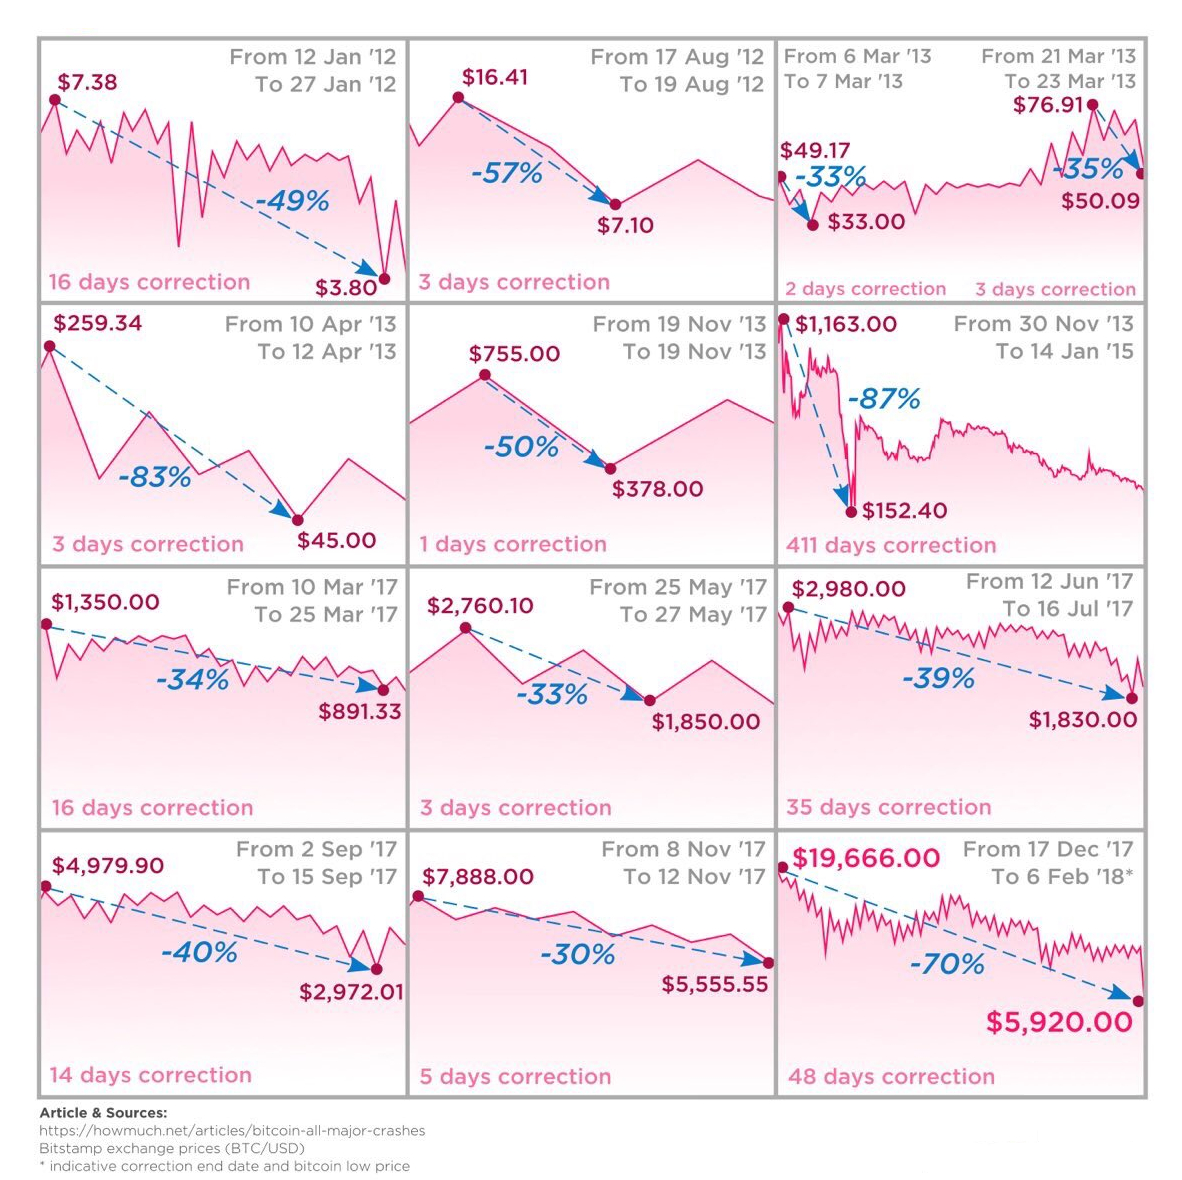
\includegraphics [width = 10cm] {media/crash.jpg}
\vspace {0.5cm}
\\
E quindi sì.


\subsection {Controversie}


Il Bitcoin e le criptovalute in generale sono frequentemente soggetto di controversie. La nuova tecnologia della blockchain è criticata da molti imprenditori, e numerosissime truffe girano intorno all'anonimità della valuta (wut lol)


\subsubsection {Mt. Gox}


Mt. Gox è il primo grande sito di exchange di Bitcoin, creato a Tokyo, JP nel 2013.
Ai tempi il Bitcoin aveva un valore ben più basso del \textasciitilde9000 di oggi: il giorno in cui l'hack è avvenuto un bitcoin valeva "solo" \euro{}500.


\subsubsection {Bitconnect}


Bitconnect è un altcoin con un tasso di interesse variabile (dal 0.1\% all'1\%) che aumentava quotidianamente i profitti di chiunque ne possedesse.
Non era ben chiaro chi fosse il creatore, e molti erano già dubiosi del claim di arricchire magicamente chiunque ne comprasse.
Nel .. 2017 il prezzo di Bitconnect è crollato da X a Y. Si è scoperto che l'intero progetto Bitconnect non era altro che un' "exit scam", una truffa in cui i truffatori spariscono improvvisamente, lasciando gli investitori a mani vuote.
In particolare Bitconenct è stato uno schema Ponzi, un tipo di truffa in cui il truffatore promette guadagni a chiunque si indebitasse con lui, per poi sparire.
Il nome Ponzi deriva da Charles Ponzi, un italo-americano che si arricchì notevolmetne negli anni '30(??????) compiendo ripetutamente questo tipo di truffa.
Oggi tutti coloro coinvolti nel pubblicizzare Bitconnect, soprattutto Youtuber (spiegare chi sono?) sono sotto investigazione


\section {Non solo Bitcoin}


Esistono numerosissime criptovalute. Il sito https://coinmarketcap.com ne lista ben 1640. Ritengo indispensabile spendere almeno qualche pagina a discutere/?????? delle valute più rilevanti, perchè a common misconception is that Bitcoin is the only cryptocurrency. This is simply not true. Tutte le criptovalure che non sono Bitcoin prendono il nome di Altcoin, "alternative coin".


\subsection {Ethereum}


Ethereum è una valuta creata da Vitalik Buterin, uno sviluppatore slavico xd CHE PALLE

https://github.com/ethereum/wiki/wiki/White-Paper

https://www.ethereum.org/ether

https://theethereum.wiki/w/index.php/MainUNDERSCOREPage

https://www.coindesk.com/information/ethereum-smart-contracts-work/


\subsection {Litecoin}


Litecoin è una criptovaluta creata nel 2011 dallo sviluppatore Charlie Lee. L'obbiettivo di questa valuta è quello di comportarsi come l'argento fa con l'oro  /  se bitcon è l'oro, ltc è l'argento.
Come per questi metalli, infatti, l'oro è usato come uno "store of value", una riserva di valore, essendo un metallo prezioso con elevato valore (oggi circa \euro{}42 per grammo). L'argento è un metallo più comune con valore ben inferiore all'oro (oggi circa \euro{}16 per grammo), usato come forma di pagamento.
Lo stesso vale per Bitcoin e Litecoin. Come abbiamo visto in precedenza la supply di btc è limitata a 21.000.000, e il valore attuale per btc è di circa \euro{}7000. Di litecoin invece ne possono esistere ben 84.000.000, e il prezzo per ltc è di \euro{}100.
Questa è la differenza principale, ma di certo non l'unica.
https://www.coindesk.com/information/comparing-litecoin-bitcoin/ adesso no sbatty

\subsection {Monero}


Monero (XMR) è un altcoin creato in Aprile 2014 che ha come prima preoccupazione quella della privacy.
Monero è l'unica criptovaluta che è completamente intracciabile. Come abbiamo visto con il Bitcoin, nella blockchain possiamo trovare informazioni su tutto quello che avviene: il bilancio di qualunque indirizzo, chi manda quanto a chi.
Con Monero tutto questo non è possibile. Mentre ha una blockchain come tutti gli altri coin, non è possibile vedere le transazioni che avvengono dall'uno all'altro indirizzo, e non è nemmeno possibile visualizzare il bilancio.
Sul sito https://moneroblocks.info, infatti, viene mostrato il seguente messaggio se si cercano informazioni legate a un indirizzo:\\

\vspace {0.5cm}
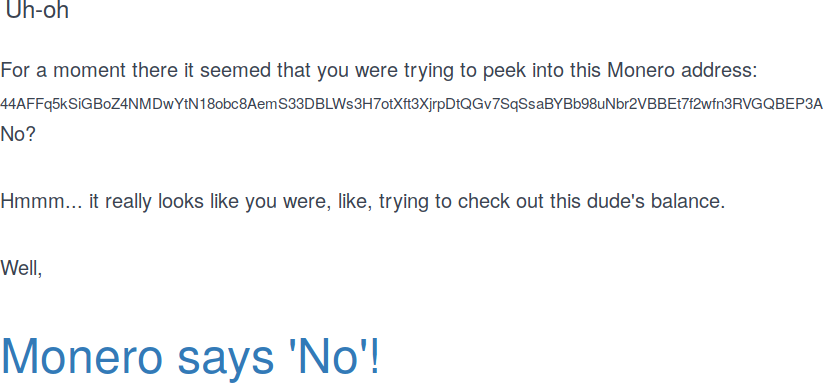
\includegraphics [width = 10cm] {media/monero.png}
\vspace {0.5cm}
\\
Questo rende Monero una valuta estremamente utile a chiunque voglia /volesse nascondere i propri fondi.
Purtroppo, come tutte le tecnologie a favore della privacy, Monero viene utilizzato anche da evasori delle tasse, truffatori e da venditori di merce illegale (V CONTROVERSIE O ADOPTION?).
Monero ha tuttavia dei limiti e non si può considerare come una valuta "perfetta": non eccelle nel campo "transazioni veloci e cheap????": in confronto al Bitcoin POST SU RMONERO BC NON TROVO INFO.


\subsection {Nano}


BEST COIN


\subsection {Ripple}


Ripple è un altcoin che è brutto perche legato alle banche centralizzato il 90\% è posseduto dai ricconi ma comunque riesce ad essere al terzo posto per market cap smh


\subsection {Bitcoin "hard forks"}


La blockchain del Bitcoin "originale" può essere clonata indefinitamente. Chiunque può prendere il codice sorgente del Bitcoin, applicarci qualche modifica e mandarlo "live", rendendo disponibili dei wallet al download e impiegando qualche miner per processare le transazioni del "nuovo" bitcoin.

\vspace {0.5cm}
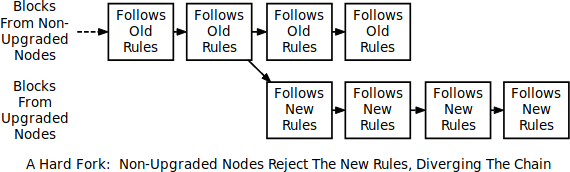
\includegraphics [width = 10cm] {media/hard_fork.png}
\vspace {0.5cm}
\\
Oggi esistono numerosissime "fork" del Bitcoin: Bitcoin Gold, Bitcoin Candy, Bitcoin Private, Bitcoin Unlimited, Bitcoin Super... Persino Bitcoin Pizza e Bitcoin God.
Quasi tutti i fork vengono visti come delle truffe, come valute che non possiedono nulla di nuovo rispetto all'originale Bitcoin, ma viene sempre data attenzione perché chiunque possiede Bitcoin il momento in cui la blockchain è stata clonata, entra automaticamente in possesso del coin della fork.
Se un indirizzo ha il bilancio di X BTC PRIMA che venga lanciato il clone di BTC, per esempio Bitcoin Top (BTT) a quell'indirizzo sarà anche associato X BTT.
Per poter ottenere effettivamente tutti i coin che l'indirizzo "possiede", è necessario scaricare il software di wallet del coin di fork e inserire la private key dell'indirizzo con su il coin di fork.
Verrà generato un nuovo indirizzo completamente diverso, però con il bilancio di X FKC.
Abbiamo visto prima che la private key dà accesso a tutti i fondi presenti sull'indirizzo a chiunque ne entri in possesso, eppure per ottenere i Fork siamo costretti ad inserirla in un software sconosciuto (perchè quasi tutti i fork non hanno alcuna reputazione: saltano fuori con siti web senza preavviso).
Per evitare che un qualche malintenzionato sfrutti la sbadataggine dell'utente e rubi tutti i suoi bitcoin, è bene che I fondi vengano mossi a un altro indirizzo.
Infatti, sarà comunque possibile prelevare i fkc dal vecchio indirizzo ora svuotato, e non si ha nulla da perdere se qualcuno riesce a rubarci la private key: l'indirizzo ha su 0 BTC.


\subsubsection {Roger Ver e la truffa di "Bitcoin Cash"}


Bitcoin Cash è by far l'hard fork più popolare di tutte, al quarto posto (!) in capitalizzazione di mercato. Come mai è l'unica che ha raggiunto un prezzo così elevato?
Roger K. Ver è un imprenditore americano che fin dai primi anni della nascita del Bitcoin è stato coinvolto nella scena delle criptovalute, finanziando progetti (?) e tenendo discorsi (??).
Da Agosto 2017, però, quando è stato lanciato Bitcoin Cash, Roger è stato l'esponente principale per il / del marketing di questa valuta. BCH è nato in Cina, infatti i suoi "CEO" sono cinesi, e Roger dev'essere stato impiegato per fare propaganda a BCH.
Tutto ciò non sembra alcunché di preoccupante: è normale se un imprenditore pubblicizza i propri investimenti sperando di ricavare più guadagni, (nel caso che...) ed è normale che sviluppatori paghnio uno abile a parlare e a pubblcizzare un prodotto.
è così che funziona il marketing.
Quella di Roger, però, è una spietata propaganda anti-Bitcoin (BTC) e pro-BCH (Bitcoin Cash), che spesso e volentieri arriva alla censura, alle bugie più false e alla corruzione di persone.
La tesi base che accomuna Roger e tutti i fan di BCH (pagati o no non si sa), è quella che BCH introduce delle modifiche al codice di Bitcoin che rendono le transizioni notevolmente più veloci, sicure e con una tassa di transazione inferiore. Bitcoin Cash infatti ha come principale differenza un'incrementata dimensione del blocco (V. 1.2), che anzichè limitarsi a 1MB arriva fino a 12MB (come abbiamo visto, ogni transazione pesa tot kb. essendo il blocco più grande può farci stare più transazioni, senza "intasarsi").
Il team di sviluppatori di Bitcoin si ostina a mantenere la dimensione del blocco a 1MB, perchè i blocchi di maggiore dimensioni sono *ancora* più difficili da minare.
Una difficoltà così elevata di mining porta necessariamente a una centralizzazione dell'hashing power, che va contro il concetto di Bitcoin e di criptovalute in generale (valute decentralizzate, internazionali, v 1.1).
Roger è entrato in possesso del sito bitcoin.com, che su numerose pagine (tra cui quella in fig. 5) ripete come BCH è una versione aggiornata di BTC. Una cosa che irrita la stragrande maggioranza delle persone è il fatto che su bitcoin.com il Bitcoin originale, BTC, è chiamato Bitcoin Core.
Il nome Bitcoin Core, paragonato a Bitcoin Cash, fa sembrare le due valute due alternative sullo stesso livello, invece uno (BCH) è un clone dell'originale (BTC). (LAWSUIT BCH = BITCOIN)
bitcoin.com, essendo il secondo risultato su google perl la ricerca "bitcoin", ha portato molte persone nuove nel mondo delle fcriptovalòute che cercavano di acquistare dei Bitcoin ad acquistare BCH anziché BTC.
Ver possiede anche l'account twitter @bitcoin, che svolge le stesse opere di propaganda di bitcoin.com


\section {Il futuro delle criprtovalute}


Come si può vedere dalla figura (se riesco a ritrovarla), nel 2018 ci troviamo alla primissima fase dell'adozione di questa nuova tecnologia.


\end {document}
